\documentclass{article}
\usepackage{graphicx}
\usepackage{fullpage}
\usepackage{amsmath}

%% Noindent file
\setlength\parindent{0pt}

\begin{document}
  \title{Beavergnaw}
  \author{Joshua T. Guerin, Ph.D.}
  
  \maketitle
  
  \begin{abstract}
    open.kattis.com problem beavergnaw\\
  \end{abstract}
  
  \begin{center}
    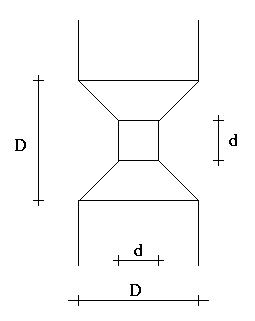
\includegraphics[width=5cm]{./images/diagram}
  \end{center}

  \section*{Relevant Formulas}
  Volume of a cylinder:
  \begin{center}
    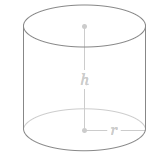
\includegraphics[width=3cm]{./images/cylinder}
  \end{center}
  \[V = \pi{}r^2h\]

  Volume of a tapered cylinder:
  \begin{center}
    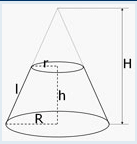
\includegraphics[width=3cm]{./images/tapered}
  \end{center}
  \[V = \dfrac{1}{3}\pi{}h(R^2 + r^2 + Rr)\]

  \section*{Problem Setup}
  To simplify the arithmetic assume:
  \[R=\dfrac{D}{2}, r=\dfrac{d}{2}\]
  These will represent the radiuses of the figures.

  
  Volume of the outer cylinder:
  \begin{align*}
    V_0 &= \pi{}R^22R\\
    &= 2\pi{}R^3\\
  \end{align*}

  Same for the inner:
  \[V_i = 2\pi{}r^3\]

  And the 2 tapered cyliners:
  \begin{align*}
    2V_t &= \dfrac{2}{3}\pi{}(R-r)(R^2 + Rr + r^2)\\\\
    &= \dfrac{2}{3}\pi{}\big(R^3 + R^2r + Rr^2 - R^2r - Rr^2 - r^3\big)\\\\
    &= \dfrac{2}{3}\pi{}\big(R^3 - r^3\big)\\
  \end{align*}

  \section*{Solution}
  Given $V$ and $D$, we have that:
  \begin{align*}
    V &= V_o - V_i - 2V_t\\
    &= 2\pi{}R^3 - 2\pi{}r^3 - \dfrac{2}{3}\pi{}\big(R^3 - r^3\big)\\
    &= 2\pi{}\bigg(R^3 - r^3 - \dfrac{1}{3}\big(R^3 - r^3\big)\bigg)\\
    &= 2\pi{}\bigg(R^3 - r^3 - \dfrac{1}{3}R^3 + \dfrac{1}{3}r^3\bigg)\\
    &= 2\pi\bigg(\dfrac{2}{3}R^3 - \dfrac{2}{3}r^3\bigg)\\
    &= 2\pi{}\dfrac{2}{3}\bigg(R^3 - r^3\bigg)\\
    &= 2\pi{}\dfrac{2}{3}\bigg(\big(\dfrac{D}{2}\big)^3 - \big(\dfrac{d}{2}\big)^3\bigg)\hspace{.5cm}\text{because } R=\dfrac{D}{2}\text{, }r=\dfrac{d}{2}\\
    &= \dfrac{2\pi{}}{3}\bigg(\dfrac{D^3}{4} - \dfrac{d^3}{4}\bigg)\\
  \end{align*}

  and so:
  \begin{align*}
    V &= \dfrac{2\pi{}}{3}\bigg(\dfrac{D^3}{4} - \dfrac{d^3}{4}\bigg)\\\\
    \dfrac{3V}{2\pi{}} &= \dfrac{D^3}{4} - \dfrac{d^3}{4}\\\\
    4\cdot \dfrac{3V}{2\pi{}} &= D^3 - d^3\\\\
    \dfrac{6V}{\pi{}} &= D^3 - d^3\\
  \end{align*}

  so:
  \[ d = \sqrt[3]{\dfrac{-6V}{\pi} + D^3} \]

  The solution is:
  \begin{center}
    \tt{print(((-6*V)/pi + D**3)**(1/3))}
  \end{center}
  
\end{document}
